\RequirePackage[l2tabu,orthodox]{nag}  % warn about common LaTeX pitfalls
\RequirePackage[ascii]{inputenc}  % input is 7-bit ASCII
\RequirePackage{fixltx2e}  % fix LaTeX2e kernel bugs

\documentclass[11pt,twoside]{article}
\usepackage{color}
\usepackage{graphicx}
\graphicspath{ {image/} }
\usepackage{calc}  % arithmetic in length parameters
\usepackage{enumitem}  % more control over list formatting
\usepackage{fancyhdr}  % simpler headers and footers
\usepackage[margin=1in]{geometry}  % page layout
\usepackage{lastpage}  % for last page number
\usepackage{relsize}  % easier font size changes
\usepackage[normalem]{ulem}  % smarter underlining
\usepackage{url}  % verb-like typesetting of URLs
%\usepackage{xfrac}  % nicer looking simple fractions for text and math
\usepackage{amsmath}
\usepackage{amssymb}

% Set up fonts.
\usepackage[T1]{fontenc}  % use true 8-bit fonts
\usepackage{slantsc}  % allow slanted small-caps
\usepackage{microtype}  % perform various font optimizations
% Use Palatino-based monospace instead of kpfonts' default.
%\usepackage{newpxtext}
\ttfamily
\DeclareFontShape{T1}{\ttdefault}{m}{scsl}{<->ssub*\ttdefault/m/sc}{}
\DeclareFontShape{T1}{\ttdefault}{b}{scsl}{<->ssub*\ttdefault/b/sc}{}
% "Kepler" fonts.
\usepackage[nott,notextcomp]{kpfonts}
% Use curvier Latin Modern brackets instead of kpfonts' glyphs.
\DeclareSymbolFont{lmsymb}     {OMS}{lmsy}{m}{n}
\DeclareSymbolFont{lmlargesymb}{OMX}{lmex}{m}{n}
\DeclareMathDelimiter{\rbrace}{\mathclose}{lmsymb}{"67}{lmlargesymb}{"09}
\DeclareMathDelimiter{\lbrace}{\mathopen}{lmsymb}{"66}{lmlargesymb}{"08}

% Page layout: stretch text to fill up page.
\addtolength\footskip{.25\headheight}
\flushbottom


% Headings.
\pagestyle{fancy}
\let\headrule\empty
\let\footrule\empty
\lhead{CSC\,336\,H1}
\chead{\large\scshape Assignment \#\ 2}
\rhead{\scshape Fall 2015}
\rfoot{\scshape ~R.J}
\lfoot{}
\cfoot{\scshape page \thepage\space of \pageref{LastPage}}
\begin{document}
\begin{enumerate}
\item
	\begin{enumerate}
		%1(a)
		\item 	%step 1
				\[ \left. \begin{bmatrix}
				1 		& \frac{1}{2} & \frac{1}{3} \\
				\frac{1}{2} & \frac{1}{3} & \frac{1}{4} \\
				\frac{1}{3} & \frac{1}{4} & \frac{1}{5} \end{bmatrix}
				 \right. 
				 \left. \begin{bmatrix}
				x_1  \\
				x_2   \\
				x_3   \end{bmatrix} \right. = \left. \begin{bmatrix}
				1  \\
				0   \\
				0   \end{bmatrix} \right.\] 
				%step 2
				\[ \left. \begin{bmatrix}
				1 &\frac{1}{2} & \frac{1}{3} \\
				0 &\frac{1}{6} & \frac{1}{6} \\
				0 &0 		      & \frac{1}{60} \end{bmatrix}
				 \right. 
				 \left. \begin{bmatrix}
				x_1  \\
				x_2   \\
				x_3   \end{bmatrix} \right. = \left. \begin{bmatrix}
				1  \\
				-1   \\
				\frac{1}{2}   \end{bmatrix} \right.\] 
				%step 3
				\[ \left. \begin{bmatrix}
				x_1  \\
				x_2   \\
				x_3   \end{bmatrix} \right. = \left. \begin{bmatrix}
				9  \\
				-36   \\
				30   \end{bmatrix} \right.\] 
		%1(b)
		\item		\[ \left. \begin{bmatrix}
				1.0 		& \frac{1}{2} & \frac{1}{3} \\
				\frac{1}{2} & \frac{1}{3} & \frac{1}{4} \\
				\frac{1}{3} & \frac{1}{4} & \frac{1}{5} \end{bmatrix}
				 \right. 
				 = 
				 \left. \begin{bmatrix}
				1    & 0.5& 0.33 \\
				0.50 & 0.33& 0.25\\
				0.33 & 0.25& 0.20\end{bmatrix}
				 \right.
				  = 
				\left. \begin{bmatrix}
				1.0\times 10^0         & 5.0 \times 10^{-1} & 3.3 \times 10^{-1} \\
				5.0 \times 10^{-1} & 3.3 \times 10^{-1} & 2.5 \times 10^{-1} \\
				3.3 \times 10^{-1}  & 2.5 \times 10^{-1} & 2.0 \times 10^{-1}\end{bmatrix}
				 \right.\]
				 
				\[ \left. \begin{bmatrix} 
				1.0 \times 10^1  \\
				0.0   \\
				0.0  \end{bmatrix} \right.  \] 
		%1(c) 
		\item		Using two decimal-digit chopped arithmetic:
				%step 1 GE
				\[\left. \begin{bmatrix}
				1.0\times 10^0         & 5.0 \times 10^{-1} & 3.3 \times 10^{-1} \\
				5.0 \times 10^{-1} & 3.3 \times 10^{-1} & 2.5 \times 10^{-1} \\
				3.3 \times 10^{-1}  & 2.5 \times 10^{-1} & 2.0 \times 10^{-1}\end{bmatrix}
				 \right.\]
				 \[ \left. \begin{bmatrix} 
				1.0 \times 10^1  \\
				0.0   \\
				0.0  \end{bmatrix} \right.  \] 
				elimination on first column:
				%step 2 GE
				\[ M_1 A = 
				\left. \begin{bmatrix}
				1.0\times 10^0         & 0.0 & 0.0 \\
				-5.0 \times 10^{-1} & 1.0\times 10^0  &0.0\\
				-3.3 \times 10^{-1}  & 0.0 & 1.0\times 10^0  \end{bmatrix}
				 \right. 
				\left. \begin{bmatrix}
				1.0\times 10^0         & 5.0 \times 10^{-1} & 3.3 \times 10^{-1} \\
				5.0 \times 10^{-1} & 3.3 \times 10^{-1} & 2.5 \times 10^{-1} \\
				3.3 \times 10^{-1}  & 2.5 \times 10^{-1} & 2.0 \times 10^{-1}\end{bmatrix}
				 \right. \]
				 \[ = 
				 \left. \begin{bmatrix}
				1.0\times 10^0 & 5.0 \times 10^{-1} & 3.3 \times 10^{-1}\\
				0.0                & 8.0 \times 10^{-2} & 9.0 \times 10^{-2} \\
				0.0                & 9.0 \times 10^{-2}  & 1.0 \times 10^{-1} \end{bmatrix}
				 \right. \]
				 
				 \[ M_1 b = 
				\left. \begin{bmatrix}
				1.0\times 10^0         & 0.0 & 0.0 \\
				-5.0 \times 10^{-1} & 1.0\times 10^0  &0.0\\
				-3.3 \times 10^{-1}  & 0.0 & 1.0\times 10^0  \end{bmatrix}
				 \right. 
				 \left. \begin{bmatrix} 
				1.0 \times 10^1  \\
				0.0   \\
				0.0  \end{bmatrix} \right. = 
				 \left. \begin{bmatrix} 
				1.0 \times 10^1  \\
				-5.0 \times 10^{-1}  \\
				-3.3 \times 10^{-1} \end{bmatrix} \right. \] 
				
				 elimination on second column:
				 %step 3 GE
				\[ M_2M_1 A = 
				\left. \begin{bmatrix}
				1.0\times 10^0         & 0.0 & 0.0 \\
				0.0 & 1.0\times 10^0  &0.0\\
				0.0& -1.1 \times 10^0  \ (\frac{9}{8})& 1.0\times 10^0  \end{bmatrix}
				 \right. 
				\left. \begin{bmatrix}
				1.0\times 10^0 & 5.0 \times 10^{-1} & 3.3 \times 10^{-1}\\
				0.0 & 8.0 \times 10^{-2} & 9.0 \times 10^{-2} \\
				0.0  & 9.0 \times 10^{-2}  & 1.0 \times 10^{-1} \end{bmatrix}
				 \right. \]
				 \[ = 
				 \left. \begin{bmatrix}
				1.0\times 10^0 & 5.0 \times 10^{-1} & 3.3 \times 10^{-1}\\
				0.0                & 8.0 \times 10^{-2} & 9.0 \times 10^{-2} \\
				0.0                & 0.0  & 1.0 \times 10^{-3} \end{bmatrix}
				 \right. \]
				 
				 \[M_2 M_1 b = 
				\left. \begin{bmatrix}
				1.0\times 10^0         & 0.0 & 0.0 \\ 
				0.0 & 1.0\times 10^0  &0.0\\
				0.0 & -1.1 \times 10^0  \ (\frac{9}{8})&1.0\times 10^0  \end{bmatrix}
				 \right. 
				 \left. \begin{bmatrix} 
				1.0 \times 10^1  \\
				-5.0 \times 10^{-1}  \\
				-3.3 \times 10^{-1} \end{bmatrix} \right. = 
				 \left. \begin{bmatrix} 
				1.0 \times 10^1  \\
				-5.0 \times 10^{-1}  \\
				2.2 \times 10^{-1} \end{bmatrix} \right. \] 
				Hence, the solution is
				\[\left. \begin{bmatrix}
				x_1  \\
				x_2   \\
				x_3   \end{bmatrix} \right. =
				\left. \begin{bmatrix} 
				3.7 \times 10^1  \\
				-2.3 \times 10^{2}  \\
				2.2 \times 10^{2} \end{bmatrix} \right. \] 
		%1(d)	
		\item		Using exact arithmetic:
				%step 1 GE
				\[\left. \begin{bmatrix}
				1    & 0.5  & 0.33  \\
				0.5 & 0.33 & 0.25  \\
				0.33 & 0.25 & 0.2 \end{bmatrix}
				 \right.\]
				 \[ \left. \begin{bmatrix} 
				1 \\
				0   \\
				0  \end{bmatrix} \right.  \] 
				 elimination on first column:
				%step 2 GE
				\[ M_1 A = 
				\left. \begin{bmatrix}
				1& 0 & 0 \\
				-5.0& 1&0\\
				-3.3& 0 &1 \end{bmatrix}
				 \right. 
				\left. \begin{bmatrix}
				1    & 0.5  & 0.33  \\
				0.5 & 0.33 & 0.25  \\
				0.33 & 0.25 & 0.2 \end{bmatrix}
				 \right. = 
				 \left. \begin{bmatrix}
				1.0 &0.5.0 & 0.33 \\
				0&0.08& 0.085 \\
				0& 0.085 & 0.0911\end{bmatrix}
				 \right.\]
				 
				 \[ M_1 b = 
				\left. \begin{bmatrix}
				1& 0 & 0 \\
				-5.0& 1&0\\
				-3.3& 0 &1 \end{bmatrix}
				 \right. 				 
				 \left. \begin{bmatrix} 
				1\\
				0   \\
				0  \end{bmatrix} \right. = 
				 \left. \begin{bmatrix} 
				1 \\
				-0.5\\
				-0.33 \end{bmatrix} \right. \] 
				
				elimination on second column: 
				 %step 3
				\[ M_2M_1 A = 
				\left. \begin{bmatrix}
				1& 0 & 0 \\
				0& 1&0\\
				0& \frac{9}{8} &1 \end{bmatrix}
				 \right. 
				 \left. \begin{bmatrix}
				1.0 &0.5.0 & 0.33 \\
				0&0.08& 0.085 \\
				0& 0.085 & 0.0911\end{bmatrix}
				 \right. = 
				 \left. \begin{bmatrix}
				1 & 0.5 &0.33\\
				0 & 0.08 & 0.085 \\
				0 & 0.0 & 0.0007875 \end{bmatrix}
				 \right.\]
				 
				 \[M_2 M_1 b = 
				\left. \begin{bmatrix}
				1& 0 & 0 \\
				0& 1&0\\
				0& \frac{9}{8} &1 \end{bmatrix}
				 \right. 
				 \left. \begin{bmatrix} 
				1 \\
				-0.5\\
				-0.33\end{bmatrix} \right. = 
				 \left. \begin{bmatrix} 
				 
				1 \\
				-0.5 \\
				0.20125  \end{bmatrix} \right. \] 

				%result 
				Then, we get result,
				\[ \left. \begin{bmatrix}
				x_1  \\
				x_2   \\
				x_3   \end{bmatrix} \right. = \left. \begin{bmatrix}
				 500/9\\
				-2500/9   \\
				2300/9   \end{bmatrix} \right.\] 

		%1(e)
		\item From the previous calculation we can see that  Precision ($t$) in floating point arithmetic has a great effect of the accuracy of a algorithm. \\
		In $c$ and $d$,  we are using the same algorithm, but since in $c$ we only have 2 digits of precision, then results is different from $d$. \\
		Also, In $a$ and $d$ even both are using exact arithmetic but since in $d$ the matrix is from two decimal-digit chopping, then we lost a lot in accuracy compare with $a$.
	\end{enumerate}
\item		
		\begin{itemize}[label = {}]
			\item In order to compute:
			\[ x = B^{-1}(C^{-1} + A)(2A + I) \omega \]
			\item We can rewrite it as:
			\[Bx = (C^{-1} + A)(2A+I)\omega\]
			\[CBx = C(C^{-1} + A)(2A+I)\omega\]
			\[CBx = (I + CA)(2A+I)\omega\]
			\item Clearly, $CB$ is a $n\times n$ matrix and $(I + CA)(2A+I)\omega$ is $n-vector$, so just
			solve the linear equation for $x$.	 
		 \end{itemize}
		 \begin{enumerate}[label = {\arabic*}]
		 \item calculate $\omega' = I\omega + 2A\omega$, which takes $2n^2 + n^2+2n^2 +n= 5n^2 +n$;
		 \item calculate $b = I\omega' + CA\omega'$, which takes $2n^2 + 2n^2+2n^2  + n= 6n^2 +n$;
		 \item use Gauss elimination to factor $C$ and $B$ into $P_BB = L_BU_B$ and $P_CC = L_CU_C$, which takes $2(\frac{2}{3}n^3 + \Theta(n^2)) = \frac{4}{3}n^3 + \Theta(n^2)$;
		 \item use forward solve to solve $L_Cy_1 = P_Cb$ for $y_1$,  which takes $n^2 + \Theta(n)$;
		 \item use backward solve to solve $U_Cy_2 = y_1$ for $y_2$,  which takes $n^2 + \Theta(n)$;
		 \item use forward solve to solve $L_By_3 = P_By_2$ for $y_3$,  which takes $n^2 + \Theta(n)$;
		 \item use backward solve to solve $U_Bx = y_3$ for $x$,  which takes $n^2 + \Theta(n)$. 
		 \end{enumerate}
		 Hence, this algorithm cost $\frac{4}{3}n^3 + \Theta(n^2)$ flops.
\item
\begin{enumerate}
	\item Gauss elimination without pivoting: 
		\[ 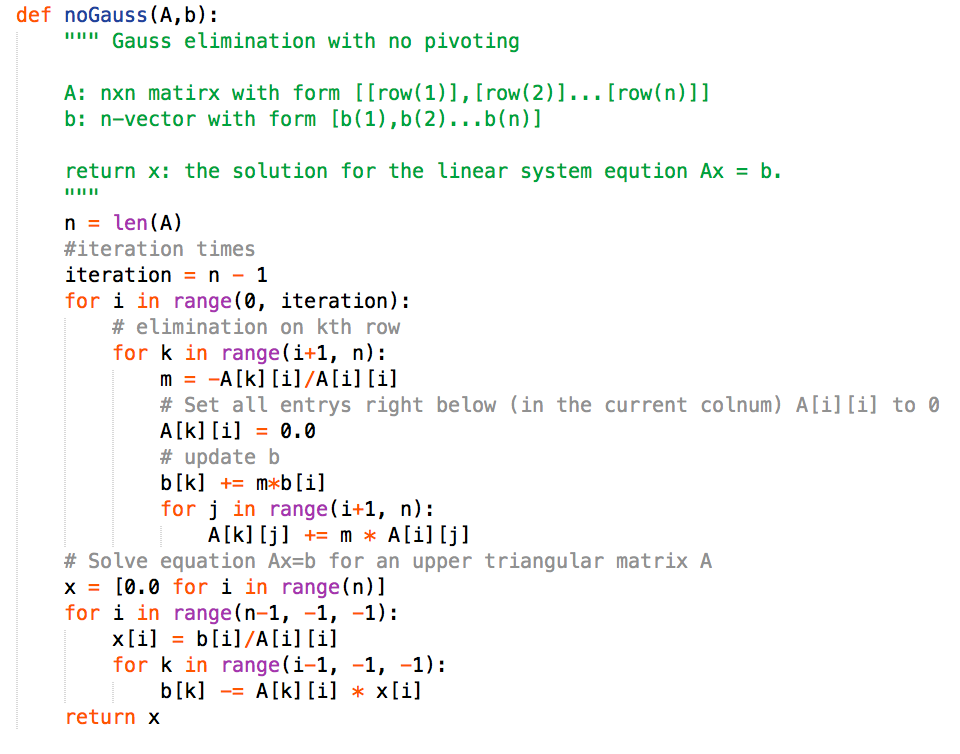
\includegraphics[scale=0.5]{ng.png} \]
		Gauss elimination with partial pivoting: 
	 	\[ 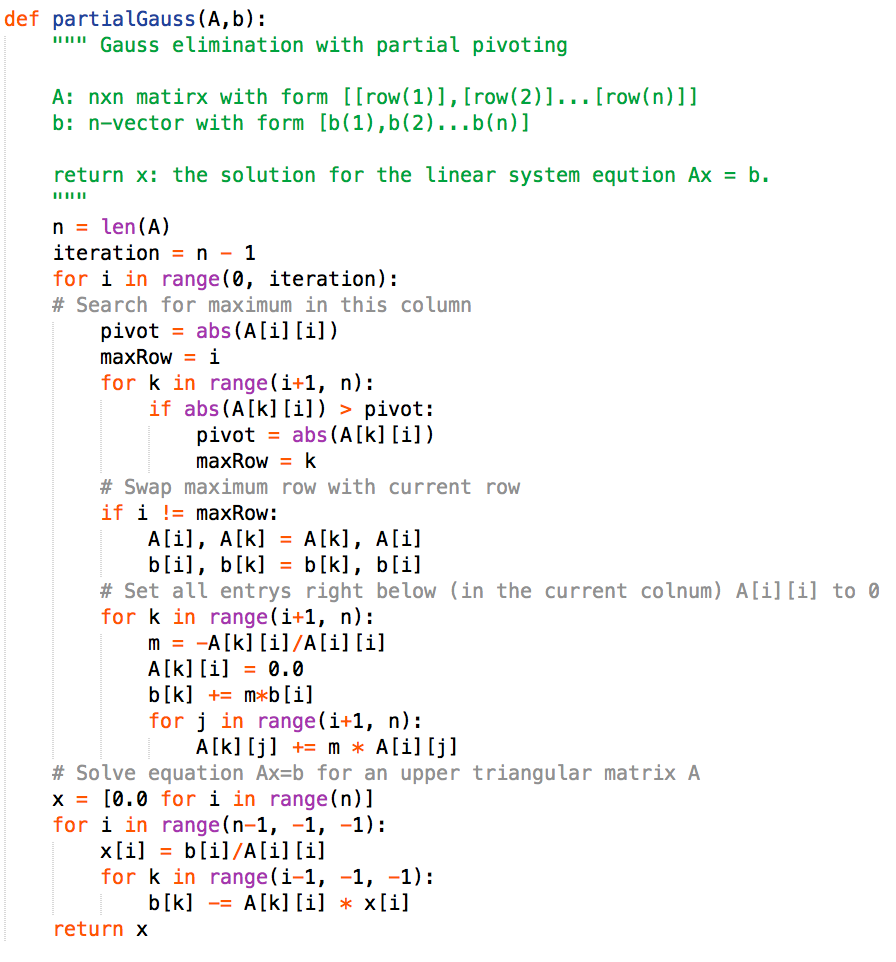
\includegraphics[scale=0.5]{pg.png} \]
		Gauss elimination complete pivoting: 
		\[ 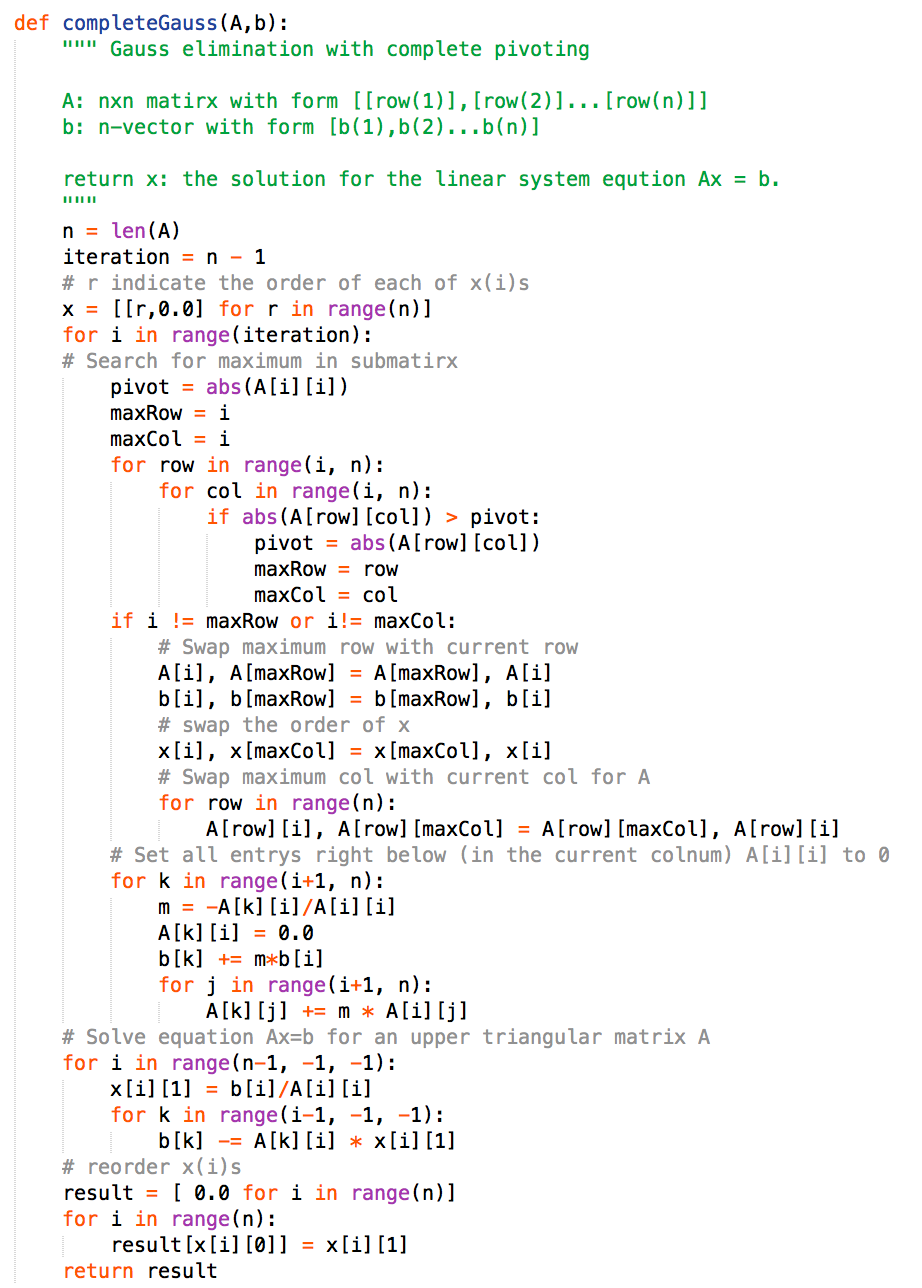
\includegraphics[scale=0.5]{cg.png} \]
	\item The function below generates random linear system equation $Ax = b$, with correct solution $x$ that $x_i = (-1)^{i+1}$
		\[ 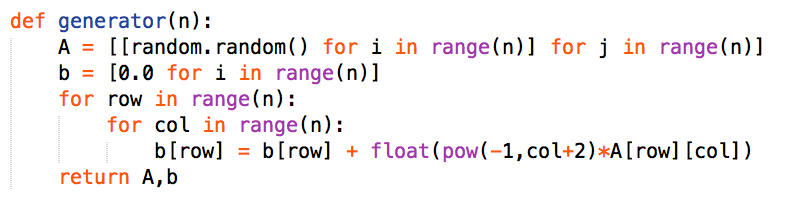
\includegraphics[scale=0.6]{generator.png} \]
		Then we randomly generates matrix of size from $1$ to $9$, the following graph shows the solutions using no pivoting, partial  pivoting, complete pivoting.
		\[ 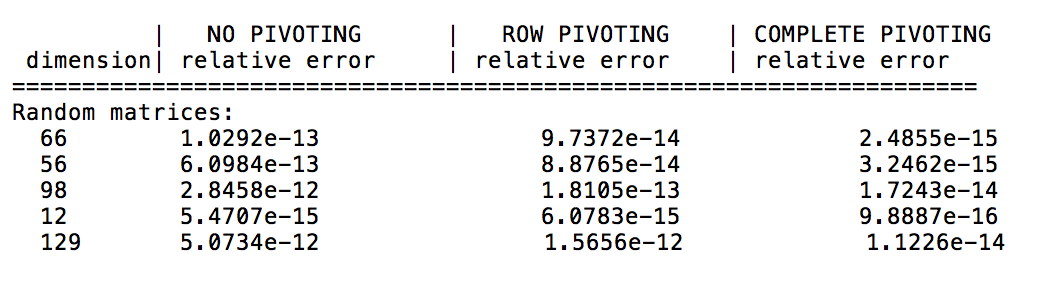
\includegraphics[scale=0.5]{results.png} \]
		Observing the results, we can get that generally complete pivoting gives the best accuracy. Partial  pivoting and no pivoting has close performance, but generally partial  pivoting is better
	\item If the matrix A has the form 
		\[ \left. \begin{bmatrix}
			a_1& 0 & 0&...&0& b_1\\
			-a_1&a_2 &0&...&0&b_2\\
			-a_1& -a_2&a_3&...&0&b_3\\
			-a_1& -a_2&-a_3&...&0&b_4\\
			&&...&&&\\
			&&&...&&\\
			-a_1&-a_2&-a_3&... &a_{n-1}&b_{n-1}\\
			-a_1&-a_2&-a_3&... &-a_{n-1}&b_{n } \end{bmatrix}\right. 
		\] 
		where $a_1, a_2,...a_{n_1}$ and $b_1, b_2 ... b_n$ are all positive and $b_i \ (0<i\leq n)$ are all bigger than 1 and  $a_i \ (0<i<n)$ are relatively small. Then as size of matrix A grows bigger complete pivoting is significantly more accurate. \\ 
		Now, suppose $a_1= a_2 = ... = a_{n_1} =1$ and $ b_1= b_2 = ...= b_n = 1$, and $Ax = b$ where exact solution is $x_i = (-1)^{i+1}$ .
		\[ \left. \begin{bmatrix}
			1& 0 & 0&...&0&1\\
			-1&1&0&...&0&1\\
			-1& -1&1&...&0&1\\
			-1& -1&-1&...&0&1\\
			&&...&&&\\
			&&&...&&\\
			-1&-1&-1&... & 1&1\\
			-1&-1&-1&... &-1&1 \end{bmatrix}\right. 
		\] 
		No we use no pivoting, partial pivoting and complete pivoting compute $Ax = b$.\\
		\[ 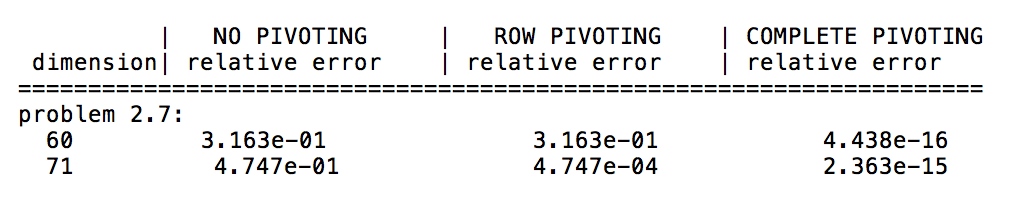
\includegraphics[scale=0.5]{3c.png} \]
\end{enumerate}
\item 
	\begin{enumerate}
	\item We know that 
		\[\frac{|| \hat {x}  - x||_{\infty}}{||x||_{\infty}} \approx cond(A)\epsilon_{mach} \]
		Then,
		\[\frac{|| \hat {x}  - x||_{\infty}}{||x||_{\infty}} \approx 10^{-8}\]
		Since $ || x||_{\infty} = 1.234567890123456789 \times10^1$, then $|| \hat {x}  - x||_{\infty} \leq 1.234567890123456789\times10^{-7}$.\\
		Then $\hat {x}$ will have probably up to $10^{-5}$ or $10^{-6}$accuracy. Then those digits
		\[ \left. \begin{bmatrix}
				\underline{12.34567} \ 8901234567890  \\
				\underline{0.00123} \ 4567890123456   \end{bmatrix} \right. \] 
		\[ \left. \begin{bmatrix}
				\underline{12.345678} \ 901234567890  \\
				\underline{0.001234} \ 567890123456   \end{bmatrix} \right. \] 
		are probability agree.
	\item We know that 
			\[\frac{|| \hat {x}  - x||}{||x||} \approx cond(A)\epsilon_{mach} \]
			We want the smallest component of $x = A\diagdown b $ has at least six significant digits of accuracy, and we the the smallest component has exponent $10^{-2}$. Hence, $|| \hat {x}  - x||$ can be at most
$10^{-8}$, but to ensure $|| \hat {x}  - x||$  be at most $10^{-8}$,  $\frac{|| \hat {x}  - x||_{\infty}}{||x||_{\infty}}$ can be at most $10^{-13}$. Therefore, machine precision must be at most $10^{-19}$.
	\end{enumerate}
\item \[ 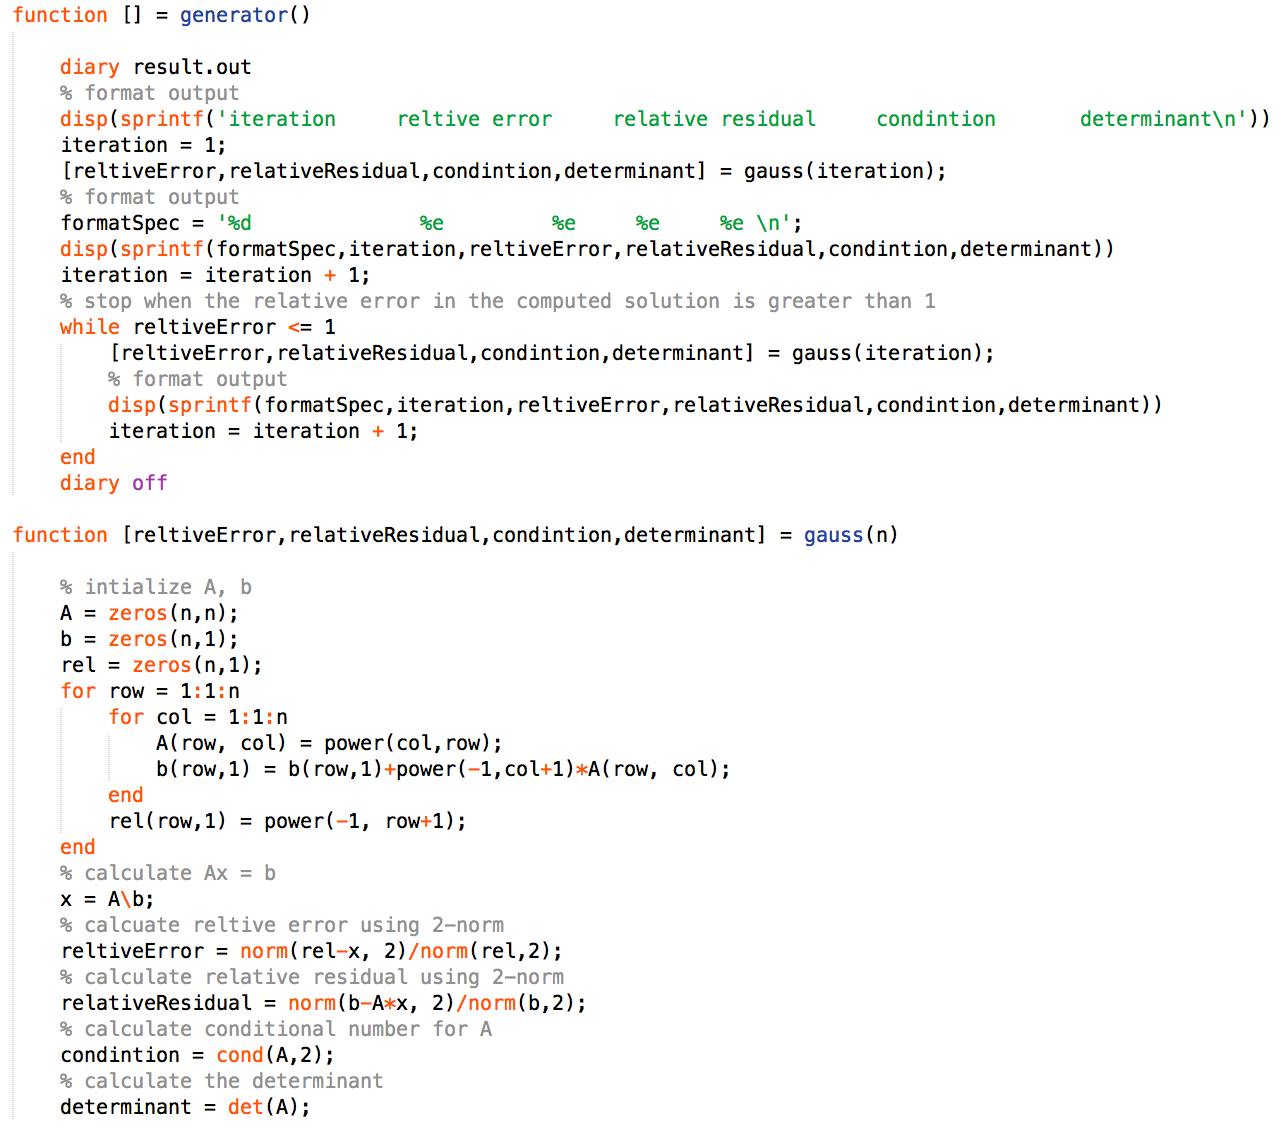
\includegraphics[scale=0.6]{mg.png} \]
	\[ 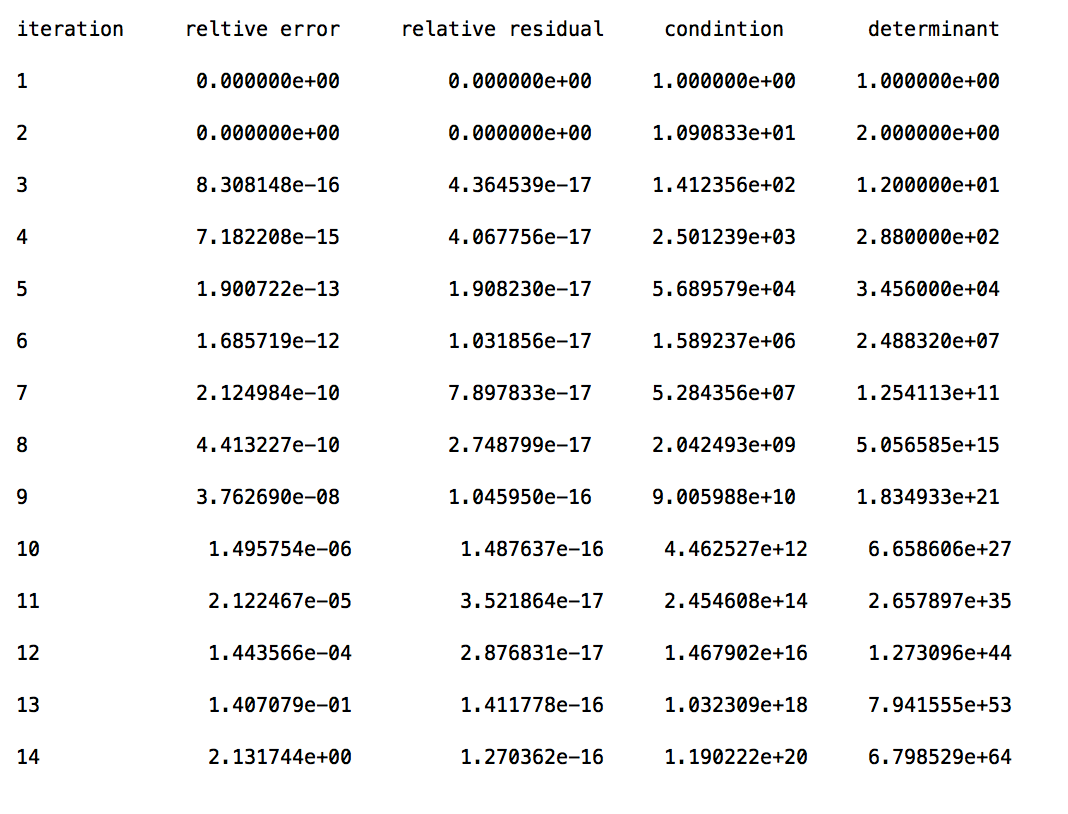
\includegraphics[scale=0.6]{mresults.png} \]
	Also, this the verification for generating the correct matrix when $n=3$:
	\[ 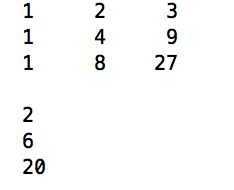
\includegraphics[scale=0.6]{verfied.png} \] 
	From the chart above we can see that, if $|det(A)|$ is big and condition number of $A$ is big as well, which means $A$ is ill condition. However,  when $|det(A)|$ is closed to $0$, $A$ is also ill condition; hence, $cond(A)$ is not always grows as $|det(A)|$ grows.
	But  from the chart we could notice that for $|det(A)| > 1$, conditional number grows as $|det(A)|$ increasing. Therefore, we know that if the  determinant is too big or determinant  is close to 0, then matrix might be ill condition.
\end{enumerate}
\end{document}
